\documentclass[11pt]{article}
\usepackage[utf8]{inputenc}
\usepackage{geometry}
\usepackage{url}
\usepackage{hyperref}
\usepackage{epsfig}
\usepackage{graphicx}
\usepackage[most]{tcolorbox}
\usepackage[export]{adjustbox}
\geometry{a4paper}
\geometry{margin=0.55in}

\usepackage[sorting=none, backend=bibtex]{biblatex}
\usepackage{filecontents}
\usepackage{tabularx}

\def\etal{\emph{et al}.\ }
\newcommand{\CPP}
{C\nolinebreak[4]\hspace{-.05em}\raisebox{.22ex}{\footnotesize\bf ++\ }}

\begin{filecontents}{final-report-references.bib}

@article{lau2016empirical,
  title={An Empirical Evaluation of doc2vec with Practical Insights into Document Embedding Generation},
  author={Lau, Jey Han and Baldwin, Timothy},
  journal={arXiv preprint arXiv:1607.05368},
  year={2016}
}

@inproceedings{mikolov2013distributed,
  title={Distributed representations of words and phrases and their compositionality},
  author={Mikolov, Tomas and Sutskever, Ilya and Chen, Kai and Corrado, Greg S and Dean, Jeff},
  booktitle={Advances in neural information processing systems},
  pages={3111--3119},
  year={2013}
}

@article{mikolov2013efficient,
  title={Efficient estimation of word representations in vector space},
  author={Mikolov, Tomas and Chen, Kai and Corrado, Greg and Dean, Jeffrey},
  journal={arXiv preprint arXiv:1301.3781},
  year={2013}
}

@inproceedings{le2014distributed,
  title={Distributed Representations of Sentences and Documents.},
  author={Le, Quoc V and Mikolov, Tomas},
  booktitle={ICML},
  volume={14},
  pages={1188--1196},
  year={2014}
}

@misc{wikidatadump2016,
  author="Meta",
  title="Data dump torrents --- Meta{,} discussion about Wikimedia projects",
  year="2016",
  url={https://meta.wikimedia.org/w/index.php?title=Data_dump_torrents},
  note="[Online; accessed 9-August-2016]"
}

@inproceedings{broder1997resemblance,
  title={On the resemblance and containment of documents},
  author={Broder, Andrei Z},
  booktitle={Compression and Complexity of Sequences 1997. Proceedings},
  pages={21--29},
  year={1997},
  organization={IEEE}
}

@misc{keras,
  title={Keras: Deep Learning library for Theano and TensorFlow},
  url={https://keras.io/}
}

@inproceedings{gensim,
  title = {{Software Framework for Topic Modelling with Large Corpora}},
  author = {Radim {\v R}eh{\r u}{\v r}ek and Petr Sojka},
  booktitle = {{Proceedings of the LREC 2010 Workshop on New
       Challenges for NLP Frameworks}},
  pages = {45--50},
  year = 2010,
  month = May,
  day = 22,
  publisher = {ELRA},
  address = {Valletta, Malta},
  note={\url{http://is.muni.cz/publication/884893/en}},
  language={English}
}

@misc{chromium2016,
  title={Git repositories on chromium},
  url={https://chromium.googlesource.com/},
  journal={chromium Git repositories}
}

@article{dai2015document,
  title={Document embedding with paragraph vectors},
  author={Dai, Andrew M and Olah, Christopher and Le, Quoc V},
  journal={arXiv preprint arXiv:1507.07998},
  year={2015}
}

@InProceedings{maas2011,
  author    = {Maas, Andrew L.  and  Daly, Raymond E.  and  Pham, Peter T.  and  Huang, Dan  and  Ng, Andrew Y.  and  Potts, Christopher},
  title     = {Learning Word Vectors for Sentiment Analysis},
  booktitle = {Proceedings of the 49th Annual Meeting of the Association for Computational Linguistics: Human Language Technologies},
  month     = {June},
  year      = {2011},
  address   = {Portland, Oregon, USA},
  publisher = {Association for Computational Linguistics},
  pages     = {142--150},
  url       = {http://www.aclweb.org/anthology/P11-1015}
}

@article{maaten2008visualizing,
  title={Visualizing data using t-SNE},
  author={Maaten, Laurens van der and Hinton, Geoffrey},
  journal={Journal of Machine Learning Research},
  volume={9},
  number={Nov},
  pages={2579--2605},
  year={2008}
}

@misc{googlegroups2015,
  title={Google Groups},
  url={https://groups.google.com/d/msg/word2vec-toolkit/q49firnoqro/bp--14e4unwj},
  journal={Google Groups}
}

@article{zhang2010understanding,
  title={Understanding bag-of-words model: a statistical framework},
  author={Zhang, Yin and Jin, Rong and Zhou, Zhi-Hua},
  journal={International Journal of Machine Learning and Cybernetics},
  volume={1},
  number={1-4},
  pages={43--52},
  year={2010},
  publisher={Springer}
}

@article{mesnil2014ensemble,
  title={Ensemble of generative and discriminative techniques for sentiment analysis of movie reviews},
  author={Mesnil, Gr{\'e}goire and Mikolov, Tomas and Ranzato, Marc'Aurelio and Bengio, Yoshua},
  journal={arXiv preprint arXiv:1412.5335},
  year={2014}
}

@article{rumelhart1988learning,
  title={Learning representations by back-propagating errors},
  author={Rumelhart, David E and Hinton, Geoffrey E and Williams, Ronald J},
  journal={Cognitive modeling},
  volume={5},
  number={3},
  pages={1},
  year={1988}
}

@article{bengio2003neural,
  title={A neural probabilistic language model},
  author={Bengio, Yoshua and Ducharme, R{\'e}jean and Vincent, Pascal and Jauvin, Christian},
  journal={journal of machine learning research},
  volume={3},
  number={Feb},
  pages={1137--1155},
  year={2003}
}

\end{filecontents}
\addbibresource{final-report-references.bib}


\title {
  \Huge Mining Big Data - Final Report\\
  \vspace{1em}
  \huge Investigating Paragraph Vectors
}

\author {
  \begin{tabular}{r l}
  a1632538 & Zachary Forman\\
  a1646930 & James Caddy\\
  \end{tabular}
}

\begin{document}

% Cover Page
\pagenumbering{gobble}
\maketitle
\newpage

\section*{Introduction}
We live in a world where enormous amounts of textual data exists, and even more
is generated each day. This data presents both a major opportunity and major
challenges, being plentiful and rich in information, but also high dimensional
and loosely structured. We can view text as consisting of words, and can
describe any collection of words as a document. In the past, textual documents
were frequently viewed as just a collection of words, the so-called
``Bag of Words" model~\cite{zhang2010understanding}. Each word in such a model
is typically just a number - the semantic connotations of words and documents
discarded for the sake of efficiency.\\
In 2013, Mikolov \etal presented the \texttt{word2vec} algorithm
~\cite{mikolov2013efficient}. This approach allowed for each word to be
represented by a vector that contains a compact representation of the
semantic meaning of that word. In 2014, Le and Mikolov extended this
approach~\cite{le2014distributed} with the \texttt{doc2vec} algorithm to
allow learning vectors that summarize the semantic meaning of a document.\\
We seek to extend Le and Mikolov's work, reproducing their \texttt{doc2vec}
results and further extending them to the domains of document similarity and
understanding source code.

\subsection*{Contributions}
This work makes the following contributions:
\begin{itemize}
  \item Replication of a relatively recent paper~\cite{le2014distributed}
        that makes some contentious claims~\cite{googlegroups2015}.
  \item Answers the age-old question of what the \emph{Citizen Kane} of
        video games is.
  \item Comparison of \texttt{doc2vec}'s suitability as a document similarity
        measure as compared to Jaccard similarity.
  \item Application of the \texttt{doc2vec} algorithm to a novel domain --
        source code.
\end{itemize}

\section*{Background}
\subsection*{Word Vectors}
The first meaningful attempt at learning vector representations was
Rumelhart \etal's 1986 contribution~\cite{rumelhart1988learning}. This work,
while relatively primitive, paved the way for more sophisticated models, such
as Bengio \etal's 2003 work~\cite{bengio2003neural}. This work presents a model
that is extremely similar to the current state of the art: Learn vectors for
words based on errors seen while trying to predict surrounding context.\\
Mikolov \etal present various enhancements to this technique
~\cite{mikolov2013efficient, mikolov2013distributed}, improving both the speed
of training the word vectors and the quality of the learned representations.
The algorithm presented in these papers is known as \texttt{word2vec}, and works
as follows (see also Figure~\ref{fig:cbow}):
\begin{enumerate}
  \item First, a set of sequential words is taken, and the central word set
        aside.
  \item This text is then projected into the vector space, and summed.
  \item The resulting vector is then used to predict the central word.
  \item The error in the prediction is backpropagated to refine both the
        estimates of the word vectors and the prediction network.
\end{enumerate}
\begin{figure}
  \centering\tcbox[nobeforeafter,minipage,width=0.45\linewidth]{
    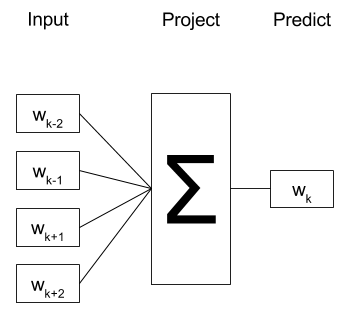
\includegraphics[width=\linewidth,left]{cbow.png}
  }
  \centering\tcbox[nobeforeafter,minipage,width=0.45\linewidth]{
    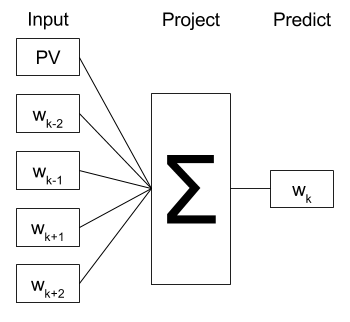
\includegraphics[width=\linewidth,right]{pbow.png}
  }
  \caption{Graphical representation of the ~\texttt{word2vec} (left)
           and ~\texttt{doc2vec} (right) algorithms.}
  \label{fig:cbow}
\end{figure}
Mikolov \etal show that these learnt word vectors not only retain semantic
information, but also relational information; for example, the result of
$\text{vec(king)} - \text{vec(man)} + \text{vec(woman)} \approx
\text{vec(queen)}$.

\subsection*{Paragraph Vectors}
In 2014, Le and Mikolov presented a method of altering the \texttt{word2vec}
algorithm to jointly train vector representations of documents in addition
to word vectors~\cite{le2014distributed}. This method is based on the idea of
basically adding a ``context vector", representing an individual document, to
each optimization. The process of learning these document vectors is equivalent
to that of learning word vectors in the \texttt{word2vec} algorithm, except an
additional paragraph vector (representing the document a given text sample comes
from) is added - see Figure~\ref{fig:cbow} for a graphical representation of the
difference. This modified \texttt{word2vec} algorithm is called
\texttt{doc2vec}.\\
Further exploration by Lau \etal shows that the \texttt{doc2vec} algorithm
provides many of the same interesting properties that \texttt{word2vec} can
provide~\cite{lau2016empirical}. Not only do the document vectors capture
semantic information, they \textit{also} capture relations: famous singers
have similar vectors, and using document vectors trained on wikipedia
pages, ``Lady Gaga" - ``America" + ``Japan" is closest to ``Ayumi Hamasaki",
a famous Japanese singer~\cite{dai2015document}.

\section*{Data Collection}

\subsection*{Data Sources}
We used three sources of data. Firstly, we use Maas' IMDB set~\cite{maas2011}
for verification and English language documents which can be found at
\url{http://ai.stanford.edu/~amaas/data/sentiment/}. Secondly, we used The
Wikimedia Foundation's English Wikipedia data dump~\cite{wikidatadump2016} as
a source for English language documents. We downloaded the full wiki dump from
\url{https://dumps.wikimedia.org/enwiki/20160820/}. Lastly, we used The
Chromium Project's Chromium repository~\cite{chromium2016} as a source for
source code documents. We cloned the repository at revision
\href{https://github.com/nwjs/chromium.src/commit/4fe31bb06cf458234d7017950a8b2b82427487c8}
{4fe31bb06cf458234d7017950a8b2b82427487c8}.

\subsection*{Data Scale}
The IMDB dataset contains a total of 100,000 files. Half are labelled as either a
positive or negative reviews, and the remainder are unlabelled. It is 346MB in size
and contains 23 million words, from a vocabulary of 90 thousand words.\\
The English Wikipedia Dataset is a single XML file, 13GB compressed and
55GB uncompressed. It contains 16 million pages, however this includes
redirects and meta-pages such as categories and portals, and therefore only
5 million of these are useful as documents. Excluding markup, this dataset contains
approximately 4 billion words.\\
The Chromium codebase is 2.6GB in size, and contains $245$ thousand files.
Of these, $23$ thousand are C and \CPP files, which contain $4.8$ million lines of
code and $608$ thousand lines of comments.

\subsection*{Data Format}
The fundamental requirements for the \texttt{doc2vec}~\cite{le2014distributed}
algorithm to work are that each document can be associated with the words in the
document, and that words in each document are just a series of words, i.e. no
excess punctuation or markup.\\
This requirement can easily be met by storing our set of documents as a newline
separated list of space separated tokens. The following example shows how a
simple document set might be transformed into this file format:\\
$$ \{\text{``My cow was sick, but now it is better."},
    \text{``Apples are nice.",
    \text{``Amazing results!"}}\} $$\\
Convert all text to lowercase and remove all punctuation:\\
$$ \{\text{``my cow was sick but now it is better"},
    \text{``apples are nice",
    \text{``amazing results"}}\} $$\\
Concatenate documents, separated by newlines:\\
\begin{align*}&\texttt{my cow was sick but now it is better}\\
&\texttt{apples are nice}\\
&\texttt{amazing results}\\\end{align*}
This format is simple to produce, simple to parse, and - given that the
\texttt{doc2vec} algorithm needs to process every word anyway - is efficient
to read. Perhaps more importantly, especially for large datasets like the
Chromium dataset, this storage format has no storage requirements in excess
of just the raw text in the files.

\subsection*{Data Processing}
To transform the data into the format previously described, some data processing
is required. All programs that we used to transform the datasets are available at
\url{https://github.com/mbd-doc2vec-team/mbd-doc2vec/tree/master/data-processing}.

\subsubsection*{IMDB Dataset}
The IMDB dataset needed minimal processing. The bulk of the work had already been
performed by the authors of the dataset. Beyond what had already been done,
punctuation, symbols and elements of markup were removed, and each document
concatenated into a file as discussed in the previous section.

\subsubsection*{Wikipedia Dataset}
The Wikipedia dataset required extensive pre-processing, with each document
needing to be parsed from the XML, and the plain text extracted from the wiki
markup. Additionally, ``fake" documents (e.g. portals, category pages) were
removed. Each wiki page was then tokenized and stored in a file as previously
stated.

\subsubsection*{Chromium Dataset}
The Chromium codebase required extensive pre-processing as well, with each \CPP
file being tokenized and having unicode characters (e.g. ¿) removed.
Unlike the other two datasets, because punctuation and uppercase/lowercase
distinctions are semantically significant in code, we retained punctuation and
the original casing in tokens.
Each comment and string literal was then tokenized as well, with punctuation
being removed from these tokens only, and the resulting tokens being stored as
discussed in the previous section. For an example of this process, the
document
\begin{align*}
&\texttt{// Frobulates the bar, in an efficient manner.}\\
&\texttt{void Frobulate(Bar \&bar);}\\
\end{align*}
would be represented by a line in the file as follows\\
\begin{align*}
\texttt{Frobulates the bar in an efficient manner void Frobulate ( Bar \& bar ) ;}
\end{align*}


\section*{Experiments}
Following are details as to how we carried out our experiments.
Full source code to do this can be found at
\url{https://github.com/mbd-doc2vec-team/mbd-doc2vec}, and full datasets
can be obtained as listed in the ``Data Sources" section of this paper.

\subsection*{IMDB Dataset}
\let\oldlabelitemi=\labelitemi
\renewcommand\labelitemi{{\boldmath$\cdot$}}
\begin{description}
  \item Preprocessing
    \begin{itemize}
      \item The entire set of 100,000 documents were processed as described
            in the previous sections, using the imdb\_cleaner.sh and filecat.sh
            scripts available at \url{https://github.com/mbd-doc2vec-team/mbd-doc2vec/blob/master/data-processing/}
    \end{itemize}
  \item Training
    \begin{itemize}
      \item One of the co-authors of the original paper, Mikolov, provided
            some guidance and recommended the use of gensim's skip-gram model
            ~\cite{gensim}, which is trained for 20 iterations on the entire
            corpus of reviews.
      \item After each iteration, the order of the documents is randomized.
      \item The parameters we used are available at \url{https://github.com/mbd-doc2vec-team/mbd-doc2vec/blob/master/doc2vec/train_imdb_embedder.py}.
    \end{itemize}
  \item Evaluation
    \begin{itemize}
      \item The training document vectors are paired with their labels and
            a logistic regression is calculated to fit the training data.
      \item Prediction of sentiment using the testing document vectors takes
            place and the accuracy of the predicted labels versus the actual
            labels is reported.
    \end{itemize}
\end{description}

\subsection*{Wikipedia Dataset}
\begin{description}
  \item Preprocessing
    \begin{itemize}
      \item The Wikipedia XML dump was processed as discussed in the Data
            Processing section, using the parsing program available at
            \url{https://github.com/mbd-doc2vec-team/mbd-doc2vec/blob/master/data-processing/wiki_parser.cc}.
    \end{itemize}
  \item Training
    \begin{itemize}
      \item The gensim~\cite{gensim} \texttt{doc2vec} implementation was used
            to train document vectors for Wikipedia as well. We used document
            vectors of dimensionality 200, a window of 8, and summed vectors
            instead of concatenating them. We removed all words that occurred
            less than 8 times for being too rare.
    \end{itemize}
  \item Evaluation
    \begin{itemize}
      \item We evaluated the quality of the semantic modeling of the
            document vectors by qualitatively considering relationships between
            document vectors.
    \end{itemize}
\end{description}

\subsection*{Chromium Dataset}
\begin{description}
  \item Preprocessing
    \begin{itemize}
      \item The entire chromium repository was processed as described in
            the previous section, using the parsing program available at
            \url{https://github.com/mbd-doc2vec-team/mbd-doc2vec/blob/master/data-processing/source_tokenizer.cc}.
    \end{itemize}
  \item Training
    \begin{itemize}
      \item The gensim~\cite{gensim} \texttt{doc2vec} implementation was used
            to train document vectors for Chromium. We used document
            vectors of dimensionality 200, a window of 8, and summed vectors
            instead of concatenating them. We removed all tokens that occured
            less than 8 times for being too rare, much as for the wikipedia dataset.
    \end{itemize}
  \item Evaluation
    \begin{itemize}
      \item To evaluate \texttt{doc2vec} on source code, we first investigated
            how well \texttt{doc2vec}'s learned document vectors performed in
            finding clusters of related source files.
      \item Secondly, we evaluated the learned word vectors performed on tokens
            in source, to see if the semantic relationships found made sense in
            the context of the codebase.
      \item Finally, we compared the quality of the similarity
            metric given by the cosine distance of adjacent document vectors.
            We compare and contrast it with the Jaccard Similarity coefficient.
    \end{itemize}
\end{description}

\renewcommand\labelitemi{\oldlabelitemi}
\section*{Results}
\subsection*{IMDB Dataset}
Through experimentation and switching from a neural network
based approach to a logistic regression, the final best accuracy
achieved whilst attempting to replicate the results was 89.4\%.\\
Being unable to replicate the results of Le and Mikolov in
\cite{le2014distributed}, some research into the result was
conducted. Many others were trying their hardest to replicate these
results, but ultimately the co-author Mikolov, who was not involved
in the experimentation found the issue.\\
This was reported in~\cite{mesnil2014ensemble}, where Mikolov
states the 92.6\% accuracy is achievable using hierarchical softmax
``only when the training and test data are not shuffled. Thus, we
consider this result to be invalid''. We therefore confirm this
non-replication.

\subsection*{Wikipedia Dataset}
Experimentation with the Wikipedia dataset reveals some remarkable
semantic connections. Table~\ref{tab:ladygaga} shows articles with semantic
contexts that most closely resemble the article describing \emph{Lady Gaga}.
Each of these pages is that of another famous singer.
\begin{table*}[h]
  \begin{center}
    \begin{tabular}{l l}
      Page name & Cosine similarity\\
      \hline
      lorde & 0.578353\\
      lana del rey & 0.574220\\
      nicki minaj & 0.571770\\
      kreesha turner & 0.568376\\
      katy perry & 0.557113\\
    \end{tabular}
  \caption{Wikipedia pages most similar to \emph{Lady Gaga}}
  \label{tab:ladygaga}
  \end{center}
\end{table*}
\\Another nice feature of representing the embedding as a vector is being able to find
A in the relationship ``X is to Y, as A is to B'' by summing the vectors for X
and B, and subtracting Y.
A simple example of how this works is to query the model for
``London is to England, as \underline{\hspace{30pt}} is to France''
\begin{verbatim}
>>> model.docvecs.most_similar([london - england + france])
(u'paris', 0.47777268290519714)
\end{verbatim}
That the model can learn such a relationship - without any knowledge of what a
capital city is explicitly being provided to it - speaks to its representative
power.\\
\emph{Citizen Kane} is a film widely and highly regarded by critics, and as such
it has become a part of popular culture to ask the question:
``What compares to the critical acclaim of \emph{Citizen Kane}
in other types of entertainment?''. To explore the Wikipedia model's embedding
of semantics, the model was applied to answer the question,
``What is the \emph{Citizen Kane} of video games?", a question widely debated
on the internet. The results of querying the model are displayed in
Table~\ref{tab:ckvg}.
\begin{table*}[h]
  \begin{center}
    \begin{tabular}{l l}
      Page name & Cosine similarity\\
      \hline
      chrono trigger & 0.555336\\
      day of the tentacle & 0.528209\\
      deus ex & 0.507725\\
      kid icarus & 0.506333\\
      sid meier's alpha centauri & 0.502858\\
    \end{tabular}
  \caption{Wikipedia pages most similar to
           \emph{Citizen Kane} $-$ \emph{Film} $+$ \emph{Video Game}}
  \label{tab:ckvg}
  \end{center}
\end{table*}
\\Each of these games has received critical acclaim, with the ``worst" of them,
\emph{Kid Icarus}, known for having a dedicated following.\\

\subsection*{Chromium Dataset}
The final application of this document vector model was to investigate the
semantic relationships it gathers when applied to source code files. The
results were mixed. Major clusters include C$^\sharp$ code, autofill code and
the WebKit rendering engine, as can be seen in Figure~\ref{fig:tsne}.
There are clearly many other clusters, but these were less well defined, and
frequently had clusters that overlapped due to image size limitations.
Reprojection into three dimensions might help with this problem, but runs into
issues when attempting to present the results in a 2-d format, e.g. here.
\begin{figure}[h]
  \centering
    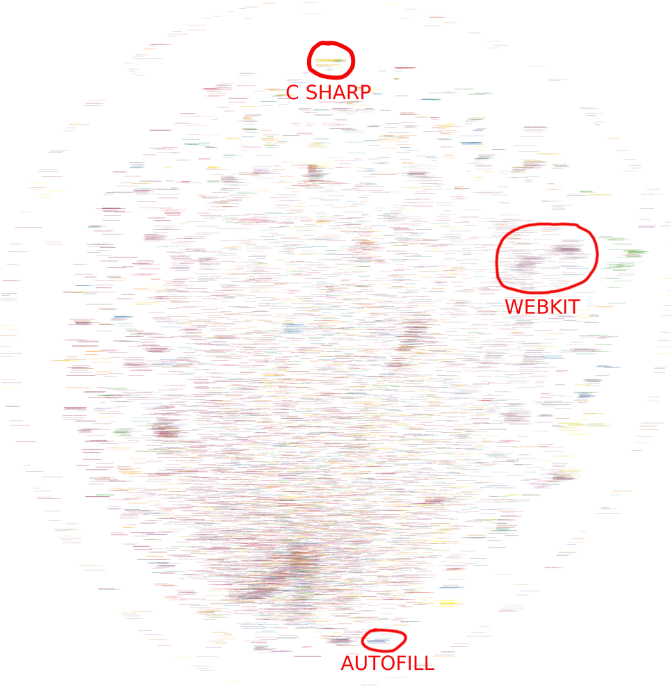
\includegraphics[width=0.5\linewidth]{chromium-tsne.png}
  \caption{t-SNE representation of the Chromium codebase under a
           \texttt{doc2vec} transform.}
  \label{fig:tsne}
\end{figure}
Otherwise, there aren't a lot of relations that can be seen in the overall
distribution.\\
Beyond these clusters, it's also interesting to see similarity patterns that
form in the tokens, as can be seen in Table~\ref{tab:chromium}. It's clear that
y, width, height, size and z are related to the idea of x as a coordinate.
\begin{table*}[h]
  \begin{center}
    \begin{tabular}{l l}
      Token & Cosine similarity\\
      \hline
      y & 0.892718\\
      width & 0.798918\\
      height & 0.762949\\
      size & 0.721175\\
      z & 0.720715\\
    \end{tabular}
  \caption{Tokens similar to $x$}
  \label{tab:chromium}
  \end{center}
\end{table*}
\\We then randomly sampled several thousand chromium files and computed the
Jaccard similarity and cosine similarity for each pair using the document vectors.
We observed that in every instance where \texttt{doc2vec} based cosine distance
indicated high semantic similarity, we found the two files to perform a similar
role. In contrast, frequently files which had a high Jaccard similarity seemed
quite dissimilar from the perspective of a software engineer. This relationship
can be seen in Figure~\ref{fig:graph}.
\begin{figure}
  \centering
    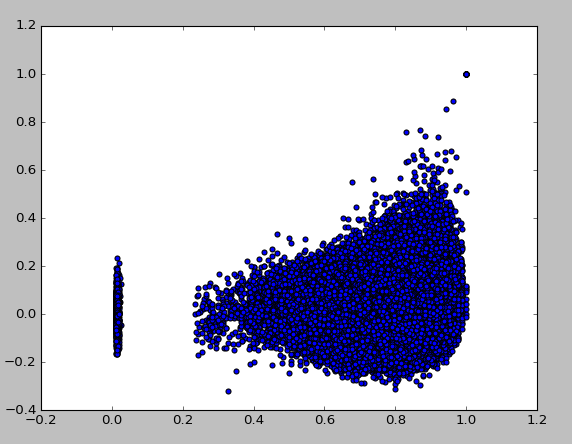
\includegraphics[width=0.5\linewidth]{js-vs-cosine.png}
  \caption{Jaccard similarity (x axis) vs Cosine similarity (y axis)}
  \label{fig:graph}
\end{figure}
\\It's clear that Jaccard similarity fails completely to find semantic
similarities on files with no words in common (see the left side of the graph),
as well as overestimating semantic similarity in much of the codebase (consider that
tokens like `+', `for', `while' will appear in almost every file, while a small
handful of tokens, like comments and variable names, will define much of the
semantic meaning of a given file).
The cost of this improved quality of similarity metric lies in the increased
time expenditure: The Jaccard similarity of a pair of documents can be computed
in tens or hundreds of microseconds - or even faster using methods like minhash.
In contrast, \texttt{doc2vec} takes order of 10s of milliseconds to infer a document
vector for an unseen document. Given that the Jaccard similarity of two documents
typically seems to serve as a useful upper bound for document similarity, however,
it might be possible to opportunistically only apply the \texttt{doc2vec} based
similarity metric to documents that are known to be somewhat similar, and achieve
both high throughput and better evaluation of semantic similarity.

\section*{Conclusion}
In this paper, we have examined the \texttt{doc2vec} algorithm.
We find that
\begin{itemize}
  \item Some of the claims made by Le and Mikolov
        in~\cite{le2014distributed}, specifically regarding accuracy
        achieved on the sentiment analysis tasks, are inaccurate, and
        reflect invalid experimental procedure as opposed to the actual
        performance of the \texttt{doc2vec} algorithm.
  \item The \emph{Citizen Kane} of video games is \emph{Chrono Trigger}.
  \item \texttt{doc2vec} with cosine similarity significantly improves
        upon Jaccard similarity in terms of evaluating the actual semantic
        similarity of two documents, but uses significantly more computing
        resources in order to do so.
  \item \texttt{doc2vec} can be applied to codebases and still produce valid,
        interesting similarity results.
\end{itemize}

\subsection*{Future Work}
We identify several major directions for future work:
\begin{itemize}
  \item More formal analysis of the actual speed and quality of
        \texttt{doc2vec} with cosine similarity is necessary. We suspect
        that use of a kd-tree might allow it to perform comparably well
        to minhashing with w-shingles for a sufficiently large set of prior
        documents.
  \item Investigating techniques like minhashing to see if they can
        successfully be augmented with a \texttt{doc2vec} based method to
        validate similar documents based on semantic similarity.
  \item Investigating whether combined corpora, e.g. training on a codebase
        and English language text, or on multiple different languages
        simultaneously, can lead to a general-purpose model that handles
        different categories of input.
\end{itemize}

\printbibliography

\end{document}
